\documentclass[12pt]{article}
\usepackage{cite}
\usepackage[a4paper]{geometry}
\usepackage{graphicx}
\usepackage[utf8]{inputenc}
\usepackage{subcaption}
\usepackage{placeins}
\usepackage{wrapfig}
\usepackage{float}
\usepackage{hyperref}
\usepackage{minted}
\usepackage[noEnd=false, indLines=false]{algpseudocodex}
\usepackage{setspace}
\usepackage{times}
\usepackage{tikzit}
% \documentclass[12pt]{article}
\usepackage{cite}
\usepackage[a4paper]{geometry}
\usepackage{graphicx}
\usepackage[utf8]{inputenc}
\usepackage{subcaption}
\usepackage{placeins}
\usepackage{wrapfig}
\usepackage{float}
\usepackage{hyperref}
\usepackage{minted}
\usepackage{amsmath}
\usepackage{mathtools}
\usepackage{algorithm}
\usepackage[noEnd=false, indLines=false]{algpseudocodex}
\usepackage{setspace}
\usepackage{times}
\usepackage{tikzit}
% \documentclass[12pt]{article}
\usepackage{cite}
\usepackage[a4paper]{geometry}
\usepackage{graphicx}
\usepackage[utf8]{inputenc}
\usepackage{subcaption}
\usepackage{placeins}
\usepackage{wrapfig}
\usepackage{float}
\usepackage{hyperref}
\usepackage{minted}
\usepackage{amsmath}
\usepackage{mathtools}
\usepackage{algorithm}
\usepackage[noEnd=false, indLines=false]{algpseudocodex}
\usepackage{setspace}
\usepackage{times}
\usepackage{tikzit}
% \documentclass[12pt]{article}
\usepackage{cite}
\usepackage[a4paper]{geometry}
\usepackage{graphicx}
\usepackage[utf8]{inputenc}
\usepackage{subcaption}
\usepackage{placeins}
\usepackage{wrapfig}
\usepackage{float}
\usepackage{hyperref}
\usepackage{minted}
\usepackage{amsmath}
\usepackage{mathtools}
\usepackage{algorithm}
\usepackage[noEnd=false, indLines=false]{algpseudocodex}
\usepackage{setspace}
\usepackage{times}
\usepackage{tikzit}
% \input{report.tikzstyles}

\graphicspath{{./images/}}

\title{Q-learning}
\author{
  Mițca Dumitru\\
  Grupa 1406A
}
\date{2025}

\begin{document}
\maketitle

\hypersetup{linkbordercolor=1 1 1}
\tableofcontents
\hypersetup{linkbordercolor=1 0 0}

\singlespacing
\newpage

\section{Proposed problem}

This year of University I have entered the NXP Cup Competition, in which me and my team must
create an autonomous car with the goal of finishing an unknown track in as little time
as possible without leaving the bounds of the tracks, which are signaled by black lines.

In this paper, I will explore the possible application of Q-Learning in this domain.

\begin{figure}
  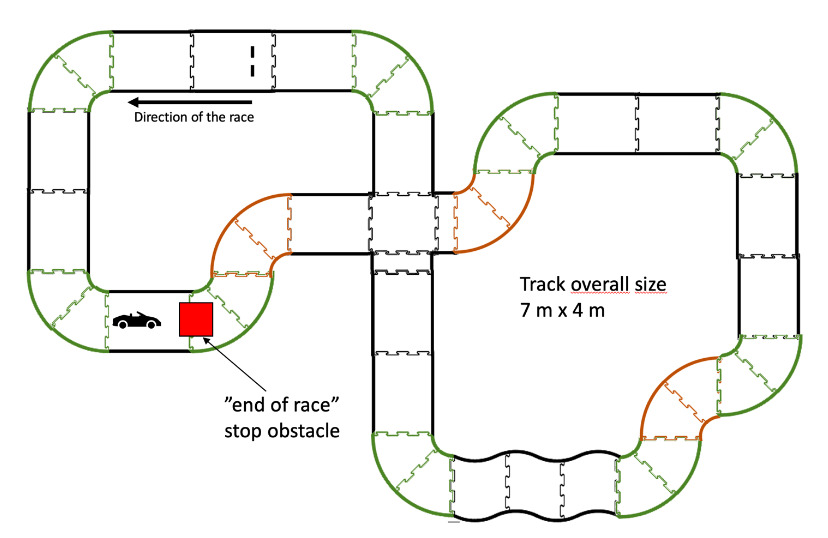
\includegraphics[width=\linewidth]{nxp-track}
  \caption{An example track\protect\footnotemark}
\end{figure}

\footnotetext{The "end of race" stop obstacle is added after the car has completed two laps} \cite[p.~9]{NxpCupRules:2025}

\newpage

\section{Algorithm}

Q-learning is a widely used reinforcement learning approach, used in domains such as game theory,
network communications, and robotics\cite{8836506}.

The goal of the agent is to maximise the total rewards it receives from the environment\cite{reinforcementlearningintro}.
\begin{align*}
  G_T = \sum_{\mathclap{k=0}}^{\infty} \gamma^{k} R_{t+k+1}
\end{align*}

We introduce a state-value function  which estimates how good being at a state $s$ is under a policy $\pi$:
\begin{align*}
  v(s) = E_{\pi}\left[\sum_{\mathclap{k=0}}^{\infty}\gamma^{k} R_{t+k+1} \mid S_t = s\right]
\end{align*}

We can then introduce an action-value function which estimates how good taking an action $a$ during a state $s$ is under a policy $\pi$:
\begin{align*}
  q(s, a) = E_{\pi}\left[\sum_{\mathclap{k=0}}^{\infty}\gamma^{k} R_{t+k+1} \mid S_t = s, A_t = a\right]
\end{align*}

We can now introduce the following Bellman equation, which our agent must maximise:
\begin{align*}
  Q(S_t, a_t) \gets (1 - \alpha) \underbrace{Q(S_t, a_t)}_{\text{current value}} + \alpha * \underbrace{(\underbrace{R_{t+1}}_{reward} + \gamma \max_{a'}{Q(S_{t+1}, a')})}_{\text{new value}}
\end{align*}

We propose the following algorithm, based on \cite[p.~67--72]{AICourse13} and \cite{qlearningalgo}:

\begin{algorithm}[H]
  \caption{Q-Learning algorithm}
  \textbf{Data:}
  \begin{itemize}
    \item $E$ --- The environment in which the agent resides
  \end{itemize}
  \textbf{Algorithm parameters:}
  \begin{itemize}
    \item $\alpha$ --- the learning rate
    \item $\gamma$ --- discount factor
    \item $\epsilon$ --- probability of exploring the environment
    \item $N_e$ --- number of episodes
    \item $N_i$ --- number of iterations per episode
  \end{itemize}
  \begin{algorithmic}
    \Procedure{QLearning}{$E$}
    \Require $\alpha, \epsilon \in \left[0, 1 \right]$, $\gamma \in \left(0, 1\right]$

    \State Initialize $Q(S, a)$, where $Q$ is a data table holding the possible reward for state $S$ and action $a$

    \For{$e \gets 0$ \textbf{to} $N_e$}
    \State $S \gets$ \Call{Reset}{$E$}

    \For{$i \gets 0$ \textbf{to} $N_i$}
    \State $a \gets$ \Call{PickAction}{$E$, $S$, $\epsilon$}
    \If{\Call{IsTerminal}{$a$}}
    \State Exit inner loop
    \EndIf
    \State take action $a$, observe reward $R$ and next state $S'$
    \State $Q(S, a) \gets (1 - \alpha)Q(S, a) + \alpha * (R + \gamma \max_{a'}{Q(S', a')})$
    \State $S \gets S'$
    \EndFor

    \EndFor

    \EndProcedure
  \end{algorithmic}
\end{algorithm}

\section{Proposed solution}
We propose to solve the problem by implementing the above algorithm in python, and creating
a text-based format for representing the map.
\section{Source code listings}

\section{Results}

\newpage

\bibliography{refs}
\bibliographystyle{ieeetr}

\section*{Individual contributions}
This project was realised solely by me, and I attest the code I have written is my own.

\end{document}


\graphicspath{{./images/}}

\title{Q-learning}
\author{
  Mițca Dumitru\\
  Grupa 1406A
}
\date{2025}

\begin{document}
\maketitle

\hypersetup{linkbordercolor=1 1 1}
\tableofcontents
\hypersetup{linkbordercolor=1 0 0}

\singlespacing
\newpage

\section{Proposed problem}

This year of University I have entered the NXP Cup Competition, in which me and my team must
create an autonomous car with the goal of finishing an unknown track in as little time
as possible without leaving the bounds of the tracks, which are signaled by black lines.

In this paper, I will explore the possible application of Q-Learning in this domain.

\begin{figure}
  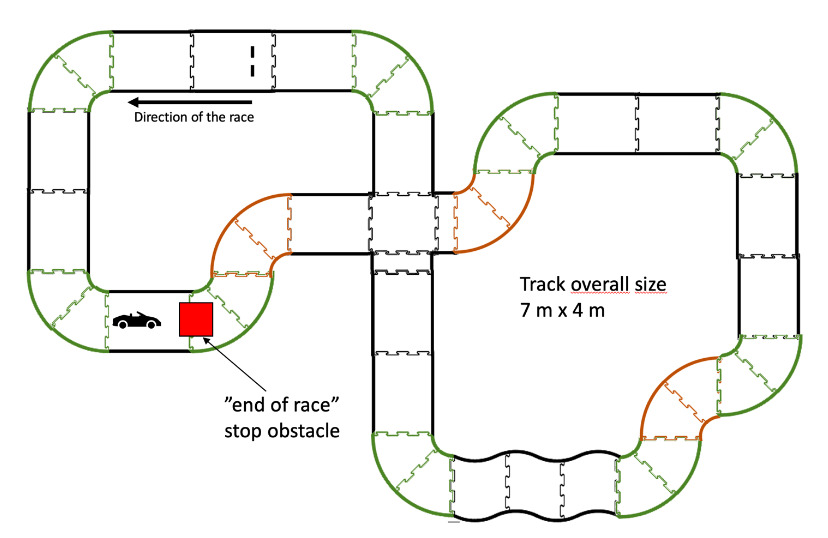
\includegraphics[width=\linewidth]{nxp-track}
  \caption{An example track\protect\footnotemark}
\end{figure}

\footnotetext{The "end of race" stop obstacle is added after the car has completed two laps} \cite[p.~9]{NxpCupRules:2025}

\newpage

\section{Algorithm}

Q-learning is a widely used reinforcement learning approach, used in domains such as game theory,
network communications, and robotics\cite{8836506}.

The goal of the agent is to maximise the total rewards it receives from the environment\cite{reinforcementlearningintro}.
\begin{align*}
  G_T = \sum_{\mathclap{k=0}}^{\infty} \gamma^{k} R_{t+k+1}
\end{align*}

We introduce a state-value function  which estimates how good being at a state $s$ is under a policy $\pi$:
\begin{align*}
  v(s) = E_{\pi}\left[\sum_{\mathclap{k=0}}^{\infty}\gamma^{k} R_{t+k+1} \mid S_t = s\right]
\end{align*}

We can then introduce an action-value function which estimates how good taking an action $a$ during a state $s$ is under a policy $\pi$:
\begin{align*}
  q(s, a) = E_{\pi}\left[\sum_{\mathclap{k=0}}^{\infty}\gamma^{k} R_{t+k+1} \mid S_t = s, A_t = a\right]
\end{align*}

We can now introduce the following Bellman equation, which our agent must maximise:
\begin{align*}
  Q(S_t, a_t) \gets (1 - \alpha) \underbrace{Q(S_t, a_t)}_{\text{current value}} + \alpha * \underbrace{(\underbrace{R_{t+1}}_{reward} + \gamma \max_{a'}{Q(S_{t+1}, a')})}_{\text{new value}}
\end{align*}

We propose the following algorithm, based on \cite[p.~67--72]{AICourse13} and \cite{qlearningalgo}:

\begin{algorithm}[H]
  \caption{Q-Learning algorithm}
  \textbf{Data:}
  \begin{itemize}
    \item $E$ --- The environment in which the agent resides
  \end{itemize}
  \textbf{Algorithm parameters:}
  \begin{itemize}
    \item $\alpha$ --- the learning rate
    \item $\gamma$ --- discount factor
    \item $\epsilon$ --- probability of exploring the environment
    \item $N_e$ --- number of episodes
    \item $N_i$ --- number of iterations per episode
  \end{itemize}
  \begin{algorithmic}
    \Procedure{QLearning}{$E$}
    \Require $\alpha, \epsilon \in \left[0, 1 \right]$, $\gamma \in \left(0, 1\right]$

    \State Initialize $Q(S, a)$, where $Q$ is a data table holding the possible reward for state $S$ and action $a$

    \For{$e \gets 0$ \textbf{to} $N_e$}
    \State $S \gets$ \Call{Reset}{$E$}

    \For{$i \gets 0$ \textbf{to} $N_i$}
    \State $a \gets$ \Call{PickAction}{$E$, $S$, $\epsilon$}
    \If{\Call{IsTerminal}{$a$}}
    \State Exit inner loop
    \EndIf
    \State take action $a$, observe reward $R$ and next state $S'$
    \State $Q(S, a) \gets (1 - \alpha)Q(S, a) + \alpha * (R + \gamma \max_{a'}{Q(S', a')})$
    \State $S \gets S'$
    \EndFor

    \EndFor

    \EndProcedure
  \end{algorithmic}
\end{algorithm}

\section{Proposed solution}
We propose to solve the problem by implementing the above algorithm in python, and creating
a text-based format for representing the map.
\section{Source code listings}

\section{Results}

\newpage

\bibliography{refs}
\bibliographystyle{ieeetr}

\section*{Individual contributions}
This project was realised solely by me, and I attest the code I have written is my own.

\end{document}


\graphicspath{{./images/}}

\title{Q-learning}
\author{
  Mițca Dumitru\\
  Grupa 1406A
}
\date{2025}

\begin{document}
\maketitle

\hypersetup{linkbordercolor=1 1 1}
\tableofcontents
\hypersetup{linkbordercolor=1 0 0}

\singlespacing
\newpage

\section{Proposed problem}

This year of University I have entered the NXP Cup Competition, in which me and my team must
create an autonomous car with the goal of finishing an unknown track in as little time
as possible without leaving the bounds of the tracks, which are signaled by black lines.

In this paper, I will explore the possible application of Q-Learning in this domain.

\begin{figure}
  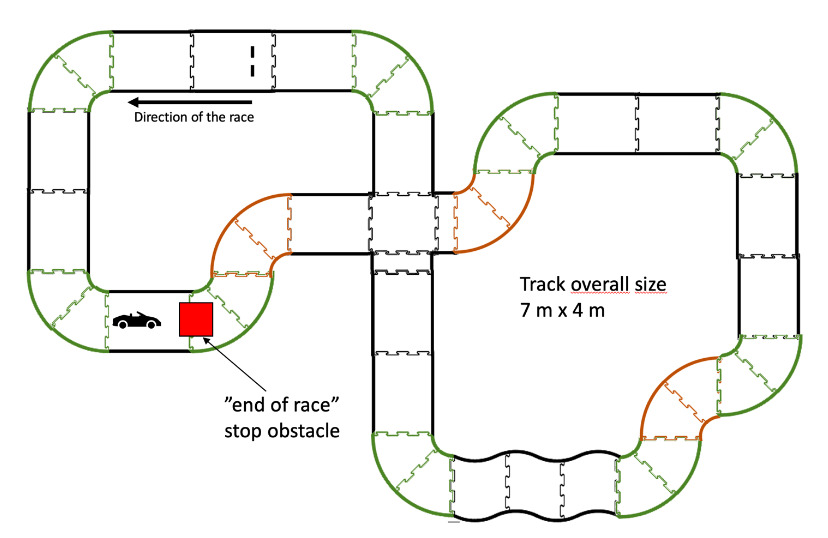
\includegraphics[width=\linewidth]{nxp-track}
  \caption{An example track\protect\footnotemark}
\end{figure}

\footnotetext{The "end of race" stop obstacle is added after the car has completed two laps} \cite[p.~9]{NxpCupRules:2025}

\newpage

\section{Algorithm}

Q-learning is a widely used reinforcement learning approach, used in domains such as game theory,
network communications, and robotics\cite{8836506}.

The goal of the agent is to maximise the total rewards it receives from the environment\cite{reinforcementlearningintro}.
\begin{align*}
  G_T = \sum_{\mathclap{k=0}}^{\infty} \gamma^{k} R_{t+k+1}
\end{align*}

We introduce a state-value function  which estimates how good being at a state $s$ is under a policy $\pi$:
\begin{align*}
  v(s) = E_{\pi}\left[\sum_{\mathclap{k=0}}^{\infty}\gamma^{k} R_{t+k+1} \mid S_t = s\right]
\end{align*}

We can then introduce an action-value function which estimates how good taking an action $a$ during a state $s$ is under a policy $\pi$:
\begin{align*}
  q(s, a) = E_{\pi}\left[\sum_{\mathclap{k=0}}^{\infty}\gamma^{k} R_{t+k+1} \mid S_t = s, A_t = a\right]
\end{align*}

We can now introduce the following Bellman equation, which our agent must maximise:
\begin{align*}
  Q(S_t, a_t) \gets (1 - \alpha) \underbrace{Q(S_t, a_t)}_{\text{current value}} + \alpha * \underbrace{(\underbrace{R_{t+1}}_{reward} + \gamma \max_{a'}{Q(S_{t+1}, a')})}_{\text{new value}}
\end{align*}

We propose the following algorithm, based on \cite[p.~67--72]{AICourse13} and \cite{qlearningalgo}:

\begin{algorithm}[H]
  \caption{Q-Learning algorithm}
  \textbf{Data:}
  \begin{itemize}
    \item $E$ --- The environment in which the agent resides
  \end{itemize}
  \textbf{Algorithm parameters:}
  \begin{itemize}
    \item $\alpha$ --- the learning rate
    \item $\gamma$ --- discount factor
    \item $\epsilon$ --- probability of exploring the environment
    \item $N_e$ --- number of episodes
    \item $N_i$ --- number of iterations per episode
  \end{itemize}
  \begin{algorithmic}
    \Procedure{QLearning}{$E$}
    \Require $\alpha, \epsilon \in \left[0, 1 \right]$, $\gamma \in \left(0, 1\right]$

    \State Initialize $Q(S, a)$, where $Q$ is a data table holding the possible reward for state $S$ and action $a$

    \For{$e \gets 0$ \textbf{to} $N_e$}
    \State $S \gets$ \Call{Reset}{$E$}

    \For{$i \gets 0$ \textbf{to} $N_i$}
    \State $a \gets$ \Call{PickAction}{$E$, $S$, $\epsilon$}
    \If{\Call{IsTerminal}{$a$}}
    \State Exit inner loop
    \EndIf
    \State take action $a$, observe reward $R$ and next state $S'$
    \State $Q(S, a) \gets (1 - \alpha)Q(S, a) + \alpha * (R + \gamma \max_{a'}{Q(S', a')})$
    \State $S \gets S'$
    \EndFor

    \EndFor

    \EndProcedure
  \end{algorithmic}
\end{algorithm}

\section{Proposed solution}
We propose to solve the problem by implementing the above algorithm in python, and creating
a text-based format for representing the map.
\section{Source code listings}

\section{Results}

\newpage

\bibliography{refs}
\bibliographystyle{ieeetr}

\section*{Individual contributions}
This project was realised solely by me, and I attest the code I have written is my own.

\end{document}


\graphicspath{{./images/}}

\title{Q-learning}
\author{
  Mițca Dumitru\\
  Grupa 1406A
}
\date{2025}

\begin{document}
\maketitle

\hypersetup{linkbordercolor=1 1 1}
\tableofcontents
\hypersetup{linkbordercolor=1 0 0}

\singlespacing
\newpage

\section{Proposed problem}

\section{Algorithm}

\cite{8836506}

\section{Proposed solution}

\section{Source code listings}

\section{Results}

\newpage

\bibliography{refs}
\bibliographystyle{ieeetr}

\section*{Individual contributions}
This project was realised solely by me, and I attest the code I have written is my own.

\end{document}
